\documentclass[12pt,a4paper,twoside]{article}

\usepackage{mystyle}

% For graphics/media
\graphicspath{{../images}}
\def\imagesdir{../images}
\def\graphsdir{../graphs_grayscale}

\def\footnoteDergachev{A.\,A.~Dergachev,~dergachev88@yandex.ru}
\def\footnoteEfimov{O.\,V.~Efimov,~efimovov@yandex.ru}
\def\footnoteSmetanina{E.\,O.~Smetanina,~jannes-2002@yandex.ru}

\begin{document}

	\thispagestyle{empty}

    % УДК: http://teacode.com/online/udc/
    % 519.633: Дифференциальные уравнения второго порядка параболического и гиперболического типов
    % 519.684: Программирование для специализированных вычислительных машин
    % 519.688: Программы и алгоритмы для решения отдельных задач на вычислительных машинах
    \noindent УДК 519.633:519.684:519.688

    \noindent \textbf{ОБЗОР И СРАВНИТЕЛЬНЫЙ АНАЛИЗ ПАРАЛЛЕЛЬНЫХ ЧИСЛЕННЫХ АЛГОРИТМОВ РЕШЕНИЯ НЕЛИНЕЙНОГО УРАВНЕНИЯ ШРЁДИНГЕРА}

	\vspace{1em}

    \noindent \copyright \quad 2010 г. \quad \textbf{
    	А.\,А.~Дергачёв\footnote[1]{\footnoteDergachev},
    	О.\,В.~Ефимов\footnote[2]{\footnoteEfimov},
    	Е.\,О.~Сметанина\footnote[3]{\footnoteSmetanina}
   }

	\vspace{0.5em}

    \noindent Международный учебно-научный лазерный центр МГУ имени М.В. Ломоносова \\
    119991, ГСП-1, Москва, Ленинские горы, 1, стр. 62.

	\vspace{-3em}

    \begin{abstract}
        \noindent Рассматриваются параллельные численные методы решения нелинейного уравнения квазиоптики на основе разностных схем и быстрого преобразования Фурье.
        Приводятся результаты исследования производительности рассматриваемых методов на суперкомпьютере СКИФ <<Чебышёв>> и кластере IBM BlueGene/P,
        установленных в~Московском государственном университете имени М.\,В. Ломоносова.
        Статья подготовлена по результатам обучения по специальной программе <<Суперкомпьютерные технологии>> и собственных исследований в рамках научной работы.
        
        \vspace{1em}
        
        \noindent Ключевые слова: параллельные алгоритмы, нелинейное уравнение Шрёдингера,
        эффективность распараллеливания, метод прогонки, быстрое преобразование Фурье.
        
        \vspace{1em}
        
	    \noindent \textbf{REVIEW AND COMPARATIVE ANALYSIS OF PARALLEL NUMERICAL ALGORITHMS FOR NONLINEAR SCHRODINGER EQUATION SOLVING}
		
		\vspace{1em}
		
	    \noindent \textbf{A.\,A.~Dergachev\footnotemark[1],
	    	O.\,V.~Efimov\footnotemark[2],
	    	E.\,O.~Smetanina\footnotemark[3]
	    }
		
        \vspace{1em}
 		
        \noindent Рассматриваются параллельные численные методы решения нелинейного уравнения квазиоптики на основе разностных схем и быстрого преобразования Фурье.
        Приводятся результаты исследования производительности рассматриваемых методов на суперкомпьютере СКИФ <<Чебышёв>> и кластере IBM BlueGene/P,
        установленных в~Московском государственном университете имени М.\,В. Ломоносова.
        Статья подготовлена по результатам обучения по специальной программе <<Суперкомпьютерные технологии>> и собственных исследований в рамках научной работы.
        
        \vspace{1em}
        
        \noindent Keywords: parallel algorithms, nonlinear Schrodinger equation,
        parallelization efficiency, sweep method, fast Fourier transform.
    \end{abstract}

    %\hrule

    \section{Введение}

%Ориентировочный план отчета:
%\begin{enumerate}
%    \item Введение.
%    \item Постановка задачи.
%    \item Параллельные алгоритмы решения задачи.
%    \begin{itemize}
%        \item Использование Фурье-метода.
%        \item Использование явной схемы.
%        \item Использование неявной схемы.
%    \end{itemize}
%    \item Сравнение алгоритмов.
%    \item Выводы.
%    \item Благодарности.
%    \item Список литературы.
%\end{enumerate}

Распространение мощных фемтосекундных лазерных импульсов в атмосфере сопровождается явлением филаментации, когда существенная часть энергии излучения концентрируется в <<горячих точках>> в поперечном сечении импульса, которые наблюдаются в виде тонких протяженных нитей.
Впервые светящаяся нить, или филамент, была зарегистрирована в 1965 году при фокусировке наносекундных лазерных импульсов в кювету с органическими жидкостями \cite{FirstFilament}.
С созданием фемтосекундных лазерных установок стало возможным получение протяженных (до нескольких сотен метров) филаментов при распространении излучения в газовых средах, в частности, в атмосфере.
Краткий обзор этих и других экспериментальных результатов дан в \cite{KandidovShlenovKosarevaReview2009}.

Причиной начала формирования нитей-филаментов является эффект Керра, вызывающий самофокусировку пучка в среде.
Самофокусировка имеет место, если мощность пучка превосходит некоторую критическую $P_{cr}$, зависящую как от параметров среды (линейного и нелинейного коэффициентов преломления), так и от параметров пучка (таких как длина волны излучения и радиус, а также от формы пучка, степени его осесимметричности и так далее).
С простейшей теорией самофокусировки можно ознакомиться в \cite{AkhmanovNikitin}.
Рост интенсивности останавливается в нелинейном фокусе за счет дефокусирующего действия наведенной излучением плазмы, возникающей в результате действия нескольких механизмов, прежде всего многофотонной и туннельной ионизации.
Обычно филамент формируется на оси пучка на расстоянии, соответствующем положению нелинейного фокуса для центрального, наиболее мощного временного слоя.
На его положение могут оказывать влияние такие факторы, как флуктуации показателя преломления в турбулентной атмосфере и фазовые флуктуации в начальном пучке.

\section{Постановка задачи}

В простейшем случае уравнение, описывающее самофокусировку гауссового пучка, записывается в виде:
\begin{equation}\label{MainDim}
    \left\{
	\begin{array}{rcl}
		2ik\dfrac{\partial E}{\partial z}&=&\dfrac{\partial^2 E}{\partial x^2}+
		\dfrac{\partial^2 E}{\partial y^2} + \dfrac{2k^2}{n_0}n_2\left|E\left(x,y,z\right)\right|^2E\left(x,y,z\right)\\
        \\
		E(x,y,0)&=&E_0\exp\left\{-\dfrac{x^2+y^2}{2a_0^2}\right\},\quad (x,y)\in[-l,l]^2
	\end{array}
	\right.
\end{equation}

Здесь $E\left(x,y,z\right)$ "--- напряженность электрического поля, $k$ "--- волновое число, $z$ "--- координата вдоль оси распространения лазерного пучка, $x,y$ "--- координаты в поперечном сечении, $n_0$ и $n_2$ "--- линейный и нелинейный коэффициент преломления.
В данном уравнении учтены такие физические факторы, как дифракция лазерного пучка и кубическая (по полю) нелинейность.
Таким образом, оно описывает начальный этап филаментации, а именно распространение пучка до нелинейного фокуса, когда возросшая интенсивность приведет к плазмообразованию и дефокусировке.
Эти процессы требуют введения дополнительных слагаемых в правую часть (\ref{MainDim}).
Однако численное решение нелинейного уравнения квазиоптики представляет и самостоятельный интерес.

После обезразмеривания $E=\tilde{E}\cdot E_0$, $x=\tilde{x}\cdot a_0$, $y=\tilde{y}\cdot a_0$, $z=\tilde{z}\cdot ka_0^2$ система будет выглядеть следующим образом:
\begin{equation}\label{MainNoDim}
    \left\{
	\begin{array}{rcl}
		2i\dfrac{\partial \tilde{E}}{\partial \tilde{z}}&=&\Delta_{\perp}\tilde{E} + R\left|\tilde{E}\right|^2\tilde{E}\\
        \\		\tilde{E}(\tilde{x},\tilde{y},0)&= &\exp\left\{-\dfrac{\tilde{x}^2+\tilde{y}^2}{2}\right\}, \quad (x,y)\in\left[-\dfrac{l}{a_0},\dfrac{l}{a_0}\right]^2
	\end{array}
	\right.
\end{equation}

Основные проблемы численного моделирования задачи филаментации лазерных импульсов связаны с многомасшабностью задачи.
Поперечные масштабы пучка примерно на два порядка превосходят возникающие в нем структуры.
В то же время размер расчетной сетки должен на порядок превосходить радиус пучка, чтобы границы сетки не отсекали существенные части пучка, а также, чтобы иметь некоторую <<буферную область>>, в которую могла бы расширяться низкоинтенсивная периферийная часть пучка.
В противном случае неизбежно возникновение краевых эффектов, приводящих к искажению решения.
Кроме того, на диаметр филамента должно приходиться достаточное количество точек (не менее 10), иначе резкие перепады интенсивности в окрестности филамента будут содержать слишком высокие пространственные частоты, что приведет к невыполнению критерия Найквиста, наложению частот и, как следствие, неадекватности получаемого решения.

Таким образом, количество точек в поперечном сечении достигает $10^4$ по каждой поперечной координате. Если учесть теперь, что количество временных слоев составляет величину порядка $10^2-10^3$, то общее количество точек достигает величины $10^{11}$, а потребность в оперативной памяти "--- величины порядка 100 Гб.

\section{Параллельные алгоритмы решения задачи}\label{SplitMethod}

Были предложены три метода численного решения поставленной задачи.
Один метод основан на использовании явной схемы для уравнения (\ref{MainNoDim}).
Два других предусматривают предварительное расщепление по физическим факторам.
Интегрирование нелинейного уравнения дифракции сводится к последовательному интегрированию на каждом шаге интегрирования двух уравнений: первое описывает только дифракцию, второе "--- только нелинейность.

Эти уравнения имеют вид:
\begin{equation}\label{Split}
    \left\{
	\begin{array}{rcl}
		2i\dfrac{\partial E}{\partial z}&=&\Delta_{\perp}E \\
        \\
        2i\dfrac{\partial E}{\partial z}&=&R\left|E\right|^2E
	\end{array}
	\right.
\end{equation}

Интегрирование уравнения для нелинейности не представляет проблем:
\begin{equation}\label{KerrSolution}
    E(x,y,z_i + \Delta z) = E(x,y,z_i)\exp\left(-\frac{iR}{2}\left|E(x,y,z_i)\right|^2\Delta z\right)
\end{equation}

Отметим, что поскольку нелинейность считается локальной, то есть набег фазы в точке поперечного сечения зависит только от значения интенсивности поля в этой же точки, поэтому применение метода геометрического параллелизма не вызывает проблем.

Для интегрирование уравнения дифракции была использована неявная численная схема и метод, использующий быстрое преобразование Фурье.

Шаг интегрирования по оси $z$ по мере приближения к нелинейному фокусу должен уменьшаться, поскольку рост интенсивности при самофокусировке приводит к росту нелинейного фазового набега засчет эффекта Керра.
Критерием пригодности шага был следующим:
\begin{equation}\label{StepCriterium}
    \max\limits_{x,y}\dfrac{R}{2}\left|E(z_i)\right|^2\Delta z \leqslant 0{,}01.
\end{equation}



    \subsection{Явная схема}

Уравнение (\ref{MainNoDim}) переписывается в виде:
\begin{equation}
	\Delta E(z_i)=E(z_i+\Delta z)-E(z_i)=\frac{\partial E}{\partial z}\Delta z =
    \frac{1}{2\textbf{i}}(\Delta_{\perp}E(z_i) + R |E(z_i)|^2 E) \Delta z = f(x, y, z)\Delta z
\end{equation}

Для его решения можно применять как очень нестабильный метод Эйлера,
так и заведомо более устойчивые методы из класса <<предиктор-корректор>>,
например, метод Рунге-Кутта 4-го порядка. Он состоит в последовательном вычислении
значения функции $f$ от некоторых аргументов и последующем усреднении полученного
таким образом значения приращения.
В случае, если у нас нет поперечных координат, это выглядело бы следующим образом:
\begin{equation}\label{rk4_method}
    \begin{aligned}
        k_1 & = f(E_i,t) \\
        k_2 & = f(E_i + \frac{k_1 \Delta z}{2}) \\
        k_3 & = f(E_i + \frac{k_2 \Delta z}{2}) \\
        k_4 & = f(E_i + k_3 \Delta z) \\
        E_{i+1} & = E_i + (k_1 + 2 k_2 + 2 k_3 + k_4) \Delta z /6
    \end{aligned}
\end{equation}

Соответственно, в нашем случае на каждом шаге нужно рассчитывать значение 4-х матриц $k_i[x_n,y_m]$.

Некоторые модификации данного метода используются другими исследователями этой проблемы. В целом же из-за зависимости функции $f()$ от поперечных координат(через поперечный лапласиан) делает эту схему неустойчивой для решения данной задачи. При этом из критерия Куранта-Фридрихса-Леви следует, что шаг по оси $z$ должен быть меньше чем $c(\Delta x)^{2}$, что при увеличении количества точек в поперечном сечении приводит к чрезвычайно малому шагу по $z$.
Однако это не ставит крест на алгоритме, так как он может применяться в тех случаях, когда требуется большая точность результатов и шаг заведомо должен быть довольно мал. 

    \vspace{1em}
\textbf{3.2. Метод на основе преобразования Фурье.}
\vspace{0.5em}

<<Метод Фурье>> основан на переходе к~двумерному фурье-образу матрицы поля:
\begin{equation}\label{FourierDef}
    E\left(k_x, k_y, z\right)=\iint E\left(x,y,z\right)e^{-ik_xx-ik_yy}\,dxdy
\end{equation}

Первое из уравнений системы (\ref{Split}) в фурье-представлении будет выглядеть следующим образом:
\begin{equation}\label{DiffractionFourier}
    2i\frac{\partial E\left(k_x, k_y, z\right)}{\partial z}= (-k_x^2-k_y^2)E\left(k_x, k_y, z\right)
\end{equation}
Его решение определяется формулой
\begin{equation}\label{DiffractionFourierSolve}
    E\left(k_x, k_y, z+\Delta z\right)= E\left(k_x, k_y, z\right)\exp\left\{\dfrac{i}{2}(k_x^2+k_y^2)\left|E\left(k_x, k_y, z\right)\right|^2\right\}
\end{equation}

Для выполнения быстрого преобразования Фурье использовалась свободно распространяемая библиотека FFTW (версии 2.3) \cite{FFTW}.
Подробнее c реализацией и методом создания алгоритма для FFTW можно ознакомиться в статьях \cite{FFTW2_Generator_99, FFTW1_98}.
Данная реализация БПФ предполагает ленточное распределение матрицы поля по процессам.
Кроме того, FFTW, как любое быстрое преобразование Фурье, эффективнее работает на матрицах, размеры которых являются степенями двойки.

Рассмотрим алгоритм параллельного двумерного преобразования Фурье.
Вначале выполняется быстрое фурье-преобразование по строкам.
Этот этап происходит локально на каждом процессе, поскольку процесс содержит в своей оперативной памяти всю строку матрицы.
Затем происходит транспонирование распределённой матрицы, что связано с обменами данными между всеми процессами (то есть каждый обменивается с каждым).
Далее снова выполняется быстрое фурье-преобразование по строкам, которые до транспонирования являлись столбцами.

Существенной особенностью алгоритмов БПФ является расположение полученных коэффициентов в памяти процессоров.
Для преобразования Фурье естественным является транспонированное расположение результата в памяти всех процессов.
Этому соответствует ключ \\ FFTW\_TRANSPOSED\_ORDER функции, реализующей преобразование Фурье.
Его альтернативой является ключ FFTW\_NORMAL\_ORDER, при задании которого после выполнения преобразования Фурье
проводится дополнительное транспонирование матрицы спектра.
Кроме того существует параметр указанной функции, позволяющий использование дополнительного временного массива для ускорения преобразования.
Наконец, при создании плана фурье-преобразования существует возможность оптимизировать план с целью ускорения работы функции.
Это достигается использованием ключей FFTW\_ESTIMATE (грубая оценка) и FFTW\_MEASURE (при~этом производятся замеры времени пересылок, выполняемых в фурье-преобразовании и их оптимизация).
Как показали тесты, применение этих ключей обосновано для последовательного преобразования,
тогда как для параллельной версии различие скорости расчётов при использовании и без использования этого ключа отличаются в пределах статистической ошибки.

Учёт нелинейности при использовании данного метода осуществляется в рамках описанного в разделе 3. расщепления по физическим факторам.


    \section{Неявные схемы.}

\begin{itemize}
	\item Использовать метод расщепления по физическим факторам "--- на 
	нелинейность и дифракцию с дальнейшим расщеплением дифракции на <<дифракцию по $x$>> и
	<<дифракцию по $y$>>.
	\item Для расчета дифракции использовать консервативную схему.
	\item Расчет проводить, использую метод прогонки для трехдиагональной матрицы.
	\item Использовать блочное распределение матрицы между процессами.
\end{itemize}



    \vspace{1em}
\textbf{3.4. Сводная информация о рассмотренных методах.} 
\vspace{0.5em}

\begin{table}[h!]\hspace{-1em}
\begin{tabular}{|l|l|l|l|}
    \hline
    Метод             & Количество операций & Объём пересылок & Необходимая память \\
    \hline
    Рунге-Кутты       & $O(N^2)$            & $16Np$          & $6 N^2$ \\
    \hline
    С БПФ при $N=2^k$ & $O(N^2\log(N))$     & $O(N\log(N))p$    & $N^2 \text{ или } 2 N^2$ \\
    \hline
    С неявной схемой  & $O(N^2)$            & $4Np$           & $2 N^2$ \\
    \hline
\end{tabular}
\\[1ex]
\caption{Оценки количества вычислительных операций, сетевых обращений и потребляемой памяти рассматриваемыми методами.}
\label{tab:MethodsSummary}
\end{table}

\newpage
%\vspace{1em}
\noindent \textbf{4. Результаты.}
\vspace{0.5em}

Ниже представлены результаты замеров времени работы алгоритма с использованием преобразования Фурье при различных комбинациях параметров,
выбранных для анализа их влияния на время работы программы.
Замеры времени осуществлялись на кластере СКИФ МГУ <<Чебышёв>> 10 раз в разное время суток и усреднялись.

%%%%%%%%%%%%%%%%%%%%%%%%%%%%%%%%%%%%%%%%

    \begin{figure}[h!]
        \begin{center}
            \begin{minipage}{0.45\linewidth}
                \center{Флаг FFTW\_ESTIMATE:\\ \includegraphics[width=0.95\linewidth]{\graphsdir/Skif/FFTW_compare_N512_nomeasure_2k}}
                \caption{Время работы Фурье-алгоритма в зависимости от количества процессов. Размер матрицы $512 \times 512$. }
                \label{gr:Fourier512Nomeasure}
            \end{minipage}
            \hfill
            \begin{minipage}{0.45\linewidth}
                \center{Флаг FFTW\_MEASURE:\\ \includegraphics[width=0.95\linewidth]{\graphsdir/Skif/FFTW_compare_N512_measure_2k}}
                \caption{Время работы Фурье-алгоритма в зависимости от количества процессов. Размер матрицы $512 \times 512$.}
                \label{gr:Fourier512Measure}
            \end{minipage}
        \end{center}
    \end{figure}

    \begin{figure}[h!]
        \begin{center}
            \begin{minipage}{0.45\linewidth}
                \center{\includegraphics[width=0.95\linewidth]{\graphsdir/Skif/FFTW_compare_N2048_nomeasure_2k}}
                \caption{Время работы Фурье-алгоритма в зависимости от количества процессов. Размер матрицы $2048 \times 2048$.}
                \label{gr:Fourier2048Nomeasure}
            \end{minipage}
            \hfill
            \begin{minipage}{0.45\linewidth}
                \center{\includegraphics[width=0.95\linewidth]{\graphsdir/Skif/FFTW_compare_N2048_measure_2k}}
                \caption{Время работы Фурье-алгоритма в зависимости от количества процессов. Размер матрицы $2048 \times 2048$.}
                \label{gr:Fourier2048Measure}
            \end{minipage}
        \end{center}
    \end{figure}

    \begin{figure}[h!]
        \begin{center}
            \begin{minipage}{0.45\linewidth}
                \center{\includegraphics[width=0.95\linewidth]{\graphsdir/Skif/FFTW_compare_N8192_nomeasure_2k}}
                \caption{Время работы Фурье-алгоритма в зависимости от количества процессов. Размер матрицы $8192 \times 8192$.}
                \label{gr:Fourier8192Nomeasure}
            \end{minipage}
            \hfill
            \begin{minipage}{0.45\linewidth}
                \center{\includegraphics[width=0.95\linewidth]{\graphsdir/Skif/FFTW_compare_N8192_measure_2k}}
                \caption{Время работы Фурье-алгоритма в зависимости от количества процессов. Размер матрицы $8192 \times 8192$.}
                \label{gr:Fourier8192Measure}
            \end{minipage}
        \end{center}
    \end{figure}

    \newpage

%%%%%%%%%%%%%%%%%%%%%%%%%%%%%%%%%%%%%%%%

    \begin{figure}[h!]
        \begin{center}
            \begin{minipage}{0.48\linewidth}
                \center{\includegraphics[width=0.95\linewidth]{\graphsdir/Skif/FFTW_time_nosave_all}} \\
                \caption{Время работы Фурье-алгоритма в зависимости от количества процессов. Сохранение данных в файл не производилось.}
                \label{gr:TimeFourierNosave}
            \end{minipage}
            \hfill
            \begin{minipage}{0.48\linewidth}
                \center{\includegraphics[width=0.95\linewidth]{\graphsdir/Skif/FFTW_time_withsave_all}} \\
                \caption{Время работы Фурье-алгоритма в зависимости от количества процессов. Сохранение данных в файл производилось на каждом десятом шаге.}
                \label{gr:TimeFourierSave}
            \end{minipage}
        \end{center}
    \end{figure}

    \begin{figure}[h!]
        \begin{center}
            \begin{minipage}{0.48\linewidth}
                \center{\includegraphics[width=0.95\linewidth]{\graphsdir/Skif/FFTW_acceleration_nosave_2k}} \\
                \caption{Ускорение Фурье-алгоритма в зависимости от количества процессов. Сохранение данных в файл не производилось.}
                \label{gr:SpeedupFourierNosave}
            \end{minipage}
            \hfill
            \begin{minipage}{0.48\linewidth}
                \center{\includegraphics[width=0.95\linewidth]{\graphsdir/Skif/FFTW_acceleration_withsave_2k}} \\
                \caption{Ускорение Фурье-алгоритма в зависимости от количества процессов. Сохранение данных в файл производилось на каждом десятом шаге.}
                \label{gr:SpeedupFourierSave}
            \end{minipage}
        \end{center}
    \end{figure}

    \begin{figure}[h!]
        \begin{center}
            \begin{minipage}{0.48\linewidth}
                \center{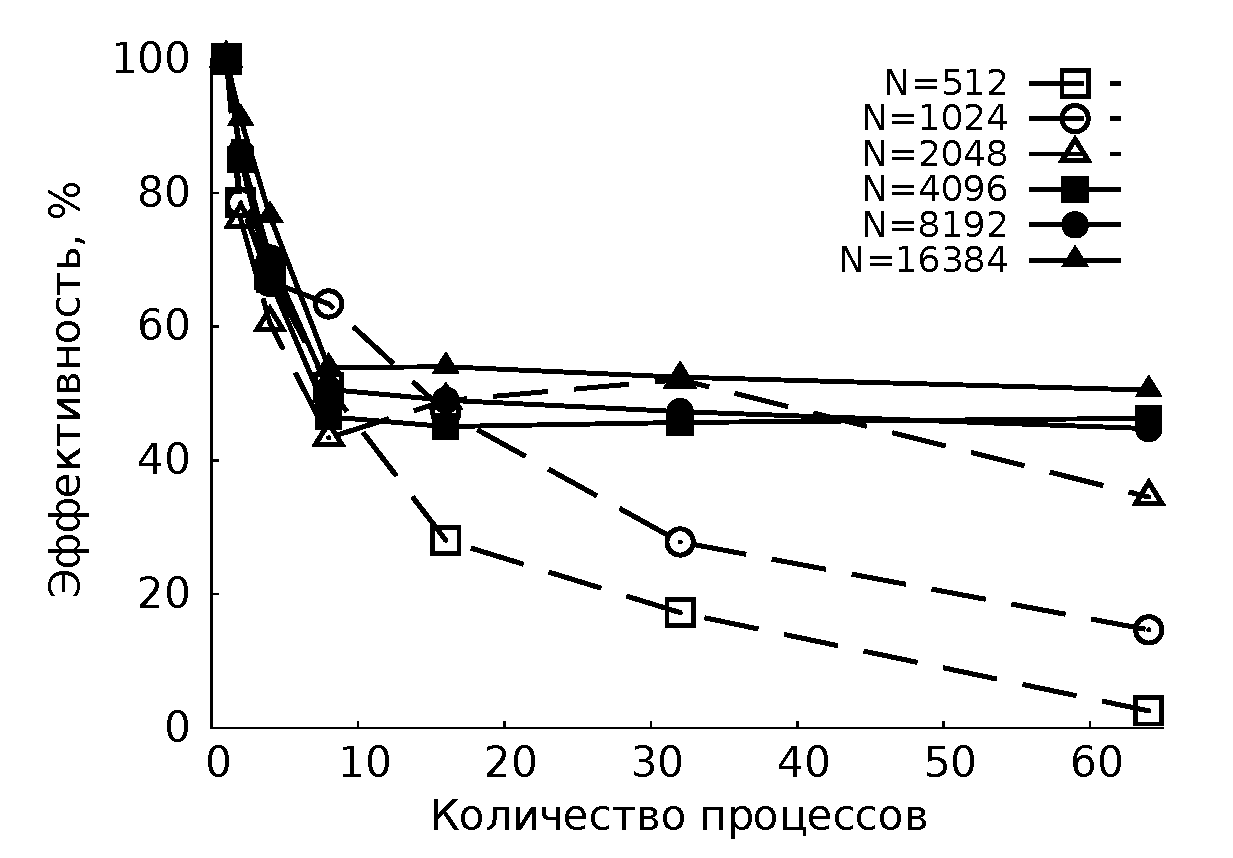
\includegraphics[width=0.95\linewidth]{\graphsdir/Skif/FFTW_efficiency_nosave_2k}} \\
                \caption{Эффективность Фурье-алгоритма в зависимости от количества процессов. Сохранение данных в файл не производилось.}
                \label{gr:EfficiencyFourierNosave}
            \end{minipage}
            \hfill
            \begin{minipage}{0.48\linewidth}
                \center{\includegraphics[width=0.95\linewidth]{\graphsdir/Skif/FFTW_efficiency_withsave_2k}} \\
                \caption{Эффективность Фурье-алгоритма в зависимости от количества процессов. Сохранение данных в файл производилось на каждом десятом шаге.}
                \label{gr:EfficiencyFourierSave}
            \end{minipage}
        \end{center}
    \end{figure}

    \newpage

%%%%%%%%%%%%%%%%%%%%%%%%%%%%%%%%%%%%%%%%

    \begin{figure}[h!]
        \begin{center}
            \begin{minipage}{0.45\linewidth}
                \center{
                    \includegraphics[width=0.95\linewidth]{\graphsdir/Skif/Sweep_time_nosave_all}
                }
                \caption{Время работы алгоритма с неявной схемой в зависимости от количества процессов. Сохранение данных в файл не производилось.}
                \label{gr:SweepTimeSkifNosave}
            \end{minipage}
            \hfill
            \begin{minipage}{0.45\linewidth}
                \center{
                    \includegraphics[width=0.95\linewidth]{\graphsdir/Skif/Sweep_time_withsave_all}
                }
                \caption{Время работы алгоритма с неявной схемой в зависимости от количества процессов. Сохранение данных в файл производилось на каждом десятом шаге.}
                \label{gr:SweepTimeSkifSave}
            \end{minipage}
        \end{center}
    \end{figure}

    \begin{figure}[h!]
        \begin{center}
            \begin{minipage}{0.45\linewidth}
                \center{
                    \includegraphics[width=0.95\linewidth]{\graphsdir/Skif/Sweep_acceleration_nosave_all}
                }
                \caption{Ускорение алгоритма с неявной схемой в зависимости от количества процессов. Сохранение данных в файл не производилось.}
                \label{gr:SweepSpeedupSkifNosave}
            \end{minipage}
            \hfill
            \begin{minipage}{0.45\linewidth}
                \center{
                    \includegraphics[width=0.95\linewidth]{\graphsdir/Skif/Sweep_acceleration_withsave_all}
                }
                \caption{Ускорение алгоритма с неявной схемой в зависимости от количества процессов. Сохранение данных в файл производилось на каждом десятом шаге.}
                \label{gr:SweepSpeedupSkifSave}
            \end{minipage}
        \end{center}
    \end{figure}

    \begin{figure}[h!]
        \begin{center}
            \begin{minipage}{0.45\linewidth}
                \center{
                    \includegraphics[width=0.95\linewidth]{\graphsdir/Skif/Sweep_efficiency_nosave_all}
                }
                \caption{Эффективность алгоритма с неявной схемой в зависимости от количества процессов. Сохранение данных в файл не производилось.}
                \label{gr:SweepEfficiencySkifNosave}
            \end{minipage}
            \hfill
            \begin{minipage}{0.45\linewidth}
                \center{
                    \includegraphics[width=0.95\linewidth]{\graphsdir/Skif/Sweep_efficiency_withsave_all}
                }
                \caption{Эффективность алгоритма с неявной схемой в зависимости от количества процессов. Сохранение данных в файл производилось на каждом десятом шаге.}
                \label{gr:SweepEfficiencySkifSave}
            \end{minipage}
        \end{center}
    \end{figure}

    \newpage

%%%%%%%%%%%%%%%%%%%%%%%%%%%%%%%%%%%%%%%%

    \begin{figure}[h!]
        \begin{center}
            \begin{minipage}{0.45\linewidth}
                \center{
                    \includegraphics[width=0.95\linewidth]{\graphsdir/Bluegene/Sweep_time_nosave_all}
                }
                \caption{Время работы алгоритма с неявной схемой на кластере IBM BlueGene/P. Сохранение данных в файл не производилось.}
                \label{gr:SweepTimeBluegeneNosave}
            \end{minipage}
            \hfill
            \begin{minipage}{0.45\linewidth}
                \center{
                    \includegraphics[width=0.95\linewidth]{\graphsdir/Bluegene/Sweep_time_withsave_all}
                }
                \caption{Время работы алгоритма с неявной схемой на кластере IBM BlueGene/P. Сохранение данных в файл производилось на каждом десятом шаге.}
                \label{gr:SweepTimeBluegeneSave}
            \end{minipage}
        \end{center}
    \end{figure}

    \begin{figure}[h!]
        \begin{center}
            \begin{minipage}{0.45\linewidth}
                \center{
                    \includegraphics[width=0.95\linewidth]{\graphsdir/Bluegene/Sweep_acceleration_nosave_all}
                }
                \caption{Ускорение параллельного алгоритма с неявной схемой на кластере IBM BlueGene/P. \mbox{Сохранение} данных в файл не производилось.}
                \label{gr:SweepSpeedupBluegeneNosave}
            \end{minipage}
            \hfill
            \begin{minipage}{0.45\linewidth}
                \center{
                    \includegraphics[width=0.95\linewidth]{\graphsdir/Bluegene/Sweep_acceleration_withsave_all}
                }
                \caption{Ускорение параллельного алгоритма с неявной схемой на кластере IBM BlueGene/P. \mbox{Сохранение} данных в файл производилось на каждом десятом шаге.}
                \label{gr:SweepSpeedupBluegeneSave}
            \end{minipage}
        \end{center}
    \end{figure}

    \begin{figure}[h!]
        \begin{center}
            \begin{minipage}{0.45\linewidth}
                \center{
                    \includegraphics[width=0.95\linewidth]{\graphsdir/Bluegene/Sweep_efficiency_nosave_all}
                }
                \caption{Эффективность параллельного алгоритма с неявной схемой на кластере IBM BlueGene/P. \mbox{Сохранение} данных в файл не производилось.}
                \label{gr:SweepEfficiencyBluegeneNosave}
            \end{minipage}
            \hfill
            \begin{minipage}{0.45\linewidth}
                \center{
                    \includegraphics[width=0.95\linewidth]{\graphsdir/Bluegene/Sweep_efficiency_withsave_all}
                }
                \caption{Эффективность параллельного алгоритма с неявной схемой на кластере IBM BlueGene/P. \mbox{Сохранение} данных в файл производилось на каждом десятом шаге.}
                \label{gr:SweepEfficiencyBluegeneSave}
            \end{minipage}
        \end{center}
    \end{figure}

    \newpage

%%%%%%%%%%%%%%%%%%%%%%%%%%%%%%%%%%%%%%%%

Из представленных на рис. \ref{gr:Fourier512Nomeasure}, \ref{gr:Fourier512Measure} графиков видно, что использование более 8 процессоров является неэффективным для матрицы размером $512\times512$,
так как время работы программы возрастает по сравнению с временем работы программы при тех же параметрах на 8 процессорах.
Для размера матрицы $2048\times2048$, как видно из рис. \ref{gr:Fourier2048Nomeasure}, \ref{gr:Fourier2048Measure} увеличение числа процессоров дает ощутимое уменьшение времени работы программы.
При использовании матрицы размером $8192\times8192$ времена работы программы увеличиваются,
что позволяет более четко увидеть различие во временах работы программы для различных комбинаций флагов при использовании библиотеки FFTW.

Из графиков на рис. \ref{gr:Fourier512Nomeasure}--\ref{gr:Fourier8192Measure} видно,
что использования флага FFTW\_MEASURE не приводит к~ускорению работы алгоритма, что связано прежде всего с малым количеством расчетных узлов.
Кроме того, использование буфера не только не привело к ускорению алгоритма, но, наоборот, несколько затормозило его.
Скорость работы алгоритма с ключом FFTW\_TRANSPOSED\_ORDER, как и ожидалось, оказалась выше, чем с ключом FFTW\_NORMAL\_ORDER.

Были проведены замеры времени для лучшего набора опций (отсутствие буфера, опции \\ FFTW\_TRANSPOSED\_ORDER и FFTW\_ESTIMATE).
Замеры проводились без сохранения матрицы в файл и с параллельной записью матрицы в файл на каждом десятом шаге.
Рассчитанные по полученным данным ускорения и эффективности программ представлены на рис. \ref{gr:SpeedupFourierNosave}--\ref{gr:EfficiencyFourierSave}.
Видно, что для размера матрицы поля, не превосходящего $2048\times2048$, использование более 8 процессов нецелесообразно, поскольку не дает прироста скорости.
Эффективность реализации резко падает для размеров матрицы поля $512\times512$ и $1024\times1024$.
Для больших матриц эффективность остается значительной: около 50\% для случая без сохранения данных и около 30\% для случая с сохранением.

Для алгоритма, использующего неявную схему, проводились замеры времени работы на суперкомпьютере СКИФ МГУ <<Чебышёв>> и кластере IBM BlueGene/P ВМиК МГУ.

Результаты замеров времени на СКИФе представлены на рис. \ref{gr:SweepSpeedupSkifNosave}--\ref{gr:SweepEfficiencySkifSave}.
Большие размеры матрицы и необходимость в дополнительной памяти для метода с использованием неявной схемы не позволили произвести расчет с использованием одного процесса,
поэтому нормировка производилась на время работы программы на 4 процессах.

Видно, что при сохранении результатов в ходе работы программы, для матриц размером $512\times512$ и $1024\times1024$ при увеличении числа процессов от 8 до 32 ускорение падает.

Эффективность работы программы при сохранении результатов в ходе работы уменьшается, относительно эффективности работы программы не сохраняющей результаты расчетов в файлы.
Увеличение числа процессов эффективно при размере матрицы более $1024\times1024$, если происходит сохранение результатов.

Результаты замеров времени работы алгоритма с использованием неявной схемы на кластере IBM Bluegene/P приведены на рис. \ref{gr:SweepTimeBluegeneNosave}--\ref{gr:SweepEfficiencyBluegeneSave}.
Видно стабильное линейное увеличение ускорения работы программы при увеличении числа процессоров уже для сравнительно небольших матриц.
Эффективность для больших рассчётных сеток превышает 60\%, что является хорошим результатом.
Таким образом, при работе на кластере IBM Bluegene/P эффективно увеличение числа процессов, на которых запускается программа.
Однако, время выполнения шага интегрирования на кластере IBM Bluegene/P существенно больше, чем на СКИФе, что связано с более слабыми процессорами.


    \cleardoublepage
\phantomsection
\section*{Заключение}
\addcontentsline{toc}{section}{Заключение}

В работе рассмотрена возможность применения пучков с регулярной поперечной структурой
для управления филаментацией лазерного импульса и проведено сравнение параметров филаментов,
образующихся при самофокусировке импульсов на длинах волн 800 нм и 10 мкм.


В частности, исследована филаментация гауссового пучка с регулярной поперечной структурой
и различными фазовыми соотношениями между соседними элементами этой структуры.

Показано, что при одинаковых остальных параметрах в случае синфазной модуляции
возникает один филамент, а в случае противофазной модуляции
возникают четыре филамента, разбегающиеся от оси распространения исходного
импульса. Величина углового расхождения филаментов определяется линейной дифракцией
пучка на~начальном этапе распространения. Обнаружено, что в случае противофазного
пучка критическая мощность самофокусировки примерно в 4 раза больше, чем в синфазном случае.
Это связано с тем, что в этом случае исходный импульс образует четыре
филамента. Таким образом, существует область значений мощности пучка, при которой
в синфазном случае филамент образуется, а в противофазном "--- нет.
Также возможен режим филаментации, при котором критическая мощность превышается уже в каждом пичке
некоторой центральной области импульса, и в таком случае они фокусируются независимо друг от друга.


Рассмотрено влияние случайных амплитудных возмущений начального пучка на~процесс
возникновения филамента и показано, что при относительной амплитуде шума
$\beta \lesssim 0.5$ они значительно не влияют на процесс формирования филаментов.


В качестве второй задачи была рассмотрена филаментация осесимметричного импульса и разработана расчётная программа, учитывающая дифракцию,
керровскую нелинейность, дисперсию второго порядка и ионизацию с учётом раздельной концентрации ионов кислорода и азота в воздухе.
Показана необходимость учёта дисперсии на этапе распространения филамента. В ходе расчётов также было получено, что для исследования распространения
сформировавшегося филамента необходимо учитывать дисперсию высших порядков и, особенно, операторы волновой нестационарности.


Проведено сравнение получающихся результатов для длины волны 800~нм с известными из литературы и показано их количественное совпадение.
Для двух импульсов с~одинаковыми длительностями, дифракционной длиной и превышением пиковой мощности над критической
при длинах волн 800~нм и 10 мкм проведено сравнение характеристик возникающего филамента и плазменного канала.
Показано, что при увеличении длины волны излучения диаметр филамента и плазменного канала увеличиваются,
тогда как концентрация плазмы уменьшается.
Это поведение предсказывается аналитическими зависимостями и экспериментальными данными,
полученными для диапазона длин волн 248--1240~нм,
что не позволяют получить количественного соответствия теоретического значения
с полученным в эксперименте для длины волны 10~мкм.
Показано, что при изменении длины волны излучения увеличивается процентное содержание ионов кислорода в образующейся плазме.


Полученные результаты могут служить основой для продолжения изучения филаментации излучения $CO_2$-лазера среднего ИК-диапазона.
Эта область длин волн на~данный момент мало исследована и может нести в себе новые интересные физические эффекты и практические приложения.


Для проведения вычислительных экспериментов был написан комплект программ
для расчёта стационарной и нестационарной задачи распространения лазерного импульса в воздухе.
В связи с тем, что часть расчётов проводилась на суперкомпьютере СКИФ МГУ <<Чебышёв>> и вычислительном кластере МЛЦ МГУ,
в процессе написания этих программ были разработаны методы распараллеливания задачи
для проведения расчётов на вычислительных кластерах и проведён сравнительный анализ параллельных численных алгоритмов решения уравнения
квазиоптики. Показано, что алгоритм на основе разностных схем имеет лучшие показатели эффективности
и масштабируемости, чем метод на основе преобразования Фурье.




    % Examples:
    % \textit{Бахвалов Н.С., Жидков Н.П., Кобельков Г.М.} Численные методы. М.: Наука, 1987.
    % Вычислительные методы линейной алгебры. Тр. I Всесоюзной конференции. Новосибирск: ВЦ СО АН СССР, 1969. 
    % \textit{Зельдович Я.Б.} К теории распространения детонации в газообразных системах // Журн. экспер. и теор. физ. 1940. 10, вып. 5. 542-568. 
    \begin{thebibliography}{99}
        \bibitem{KandidovShlenovKosarevaReview2009}%
        \textit{Кандидов В.П., Шлёнов С.А., Косарева О.Г.}
        Филаментация мощного фемтосекундного лазерного излучения.
        Квантовая электроника, 39, 3, 2009.

        \bibitem{LadaginStarikov1998}%
        \textit{Ладагин В.К., Стариков Ф.А.}
        Численное решение квазиоптического уравнения для поперечной корреляционной функции поля излучения.
        Математическое моделирование, 10, 8, 1998.

        \bibitem{Agrawal2001}%
        \textit{Agrawal G.P.}
        Applications of Nonlinear Fiber Optics (3rd edition).
        Elsevier Science, 2001.

        \bibitem{Mahankov1983}%
        \textit{Маханьков В.Г.}
        Солитоны и численный эксперимент.
        Физика элементраных частиц и атомного ядра, 14, 1, 1983.

        \bibitem{VitkovskiyFedoruk2008}%
        \textit{Витковский В.Э., Федорук М.П.}
        Численное исследование свойств решений нелинейного уравнения Шредингера при распространении лазерных импульсов в световодах.
        Вычислительные технологии, 13, 6, 2008.

        \bibitem{Kadomcev1997}%
        \textit{Кадомцев Б.Б., Кадомцев М.Б.}
        Конденсаты Бозе-Эйнштейна.
        УФН, 167, 6, 1997.

        \bibitem{Belyaeva2005}%
        \textit{Беляева Л.Т. и др.}
        Динамика солитонов в модели нелинейного уравнения Шредингера с внешним гармоническим потенциалом.
        Квантовая Электроника, 35, 9, 2005.

        \bibitem{Kartvenko1993}%
        \textit{Картавенко В.Г.}
        Линейные и нелинейные возбуждения ядерной плотности.
        Физика элементарных частиц и атомного ядра, 24, 6, 1993.

        \bibitem{Zeytunyan1995}%
        \textit{Зейтунян Р.Х.}
        Нелинейные длинные волны на поверхности воды.
        Успехи Физических Наук, 165, 12, 1995.

        \bibitem{RK_Rado_Lobatto}%
        \textit{Хайрер Э., Ваннер Г.}
        Решение обыкновенных дифференциальных уравнений. Жёсткие и дифференциально-алгебраические задачи.
        М., Мир, 1999, 685.

        \bibitem{RK_Parallel_Houwen_2001}%
        \textit{Houwen P.J., Sommeijer B.P.} Parallel ODE solver.
        // Proceedings of the International Conference on Supercomputing.
        2001, 71--81.

        \bibitem{RK_Parallel_Jackson_2001}%
        \textit{Jackson K.R., Norsett S.P.}
        The potential for parallelism in Runge-Kutta methods.Part 1: R-K formulas in standard form.
        SIAM J.Numer. Anal. 32, 2001, 49--82.

        \bibitem{FFTW}%
        http://fftw.org

        \bibitem{FFTW2_Generator_99}% This paper describes the codelet generator introduced in FFTW 2
        \textit{Matteo Frigo.} A fast Fourier transform compiler
        // Proc. 1999 ACM SIGPLAN Conf. on Programming Language Design and Implementation.
        1999. Vol. 34, num. 5, 169--180.

        \bibitem{FFTW1_98}% This was the main paper describing FFTW 1
        \textit{Matteo Frigo, Steven G. Johnson.} FFTW: An adaptive software architecture for the FFT
        // Proc. 1998 IEEE Intl. Conf. Acoustics Speech and Signal Processing.
        1998. Vol. 3, 1381--1384.

        \bibitem{Kalitkin}%
        \textit{Калиткин Н.Н.}
        Численные методы.
        М., Наука, 1978.

        \bibitem{SweepScheme}%
        \textit{V.P. Kandidov, V.Yu. Fedorov.}
        Properties of self-focusing in elliptic beams.
        Quantum Electronics, 34, 12, 2004.
    \end{thebibliography}

\end{document}
